

\begin{figure}[H]
\centering
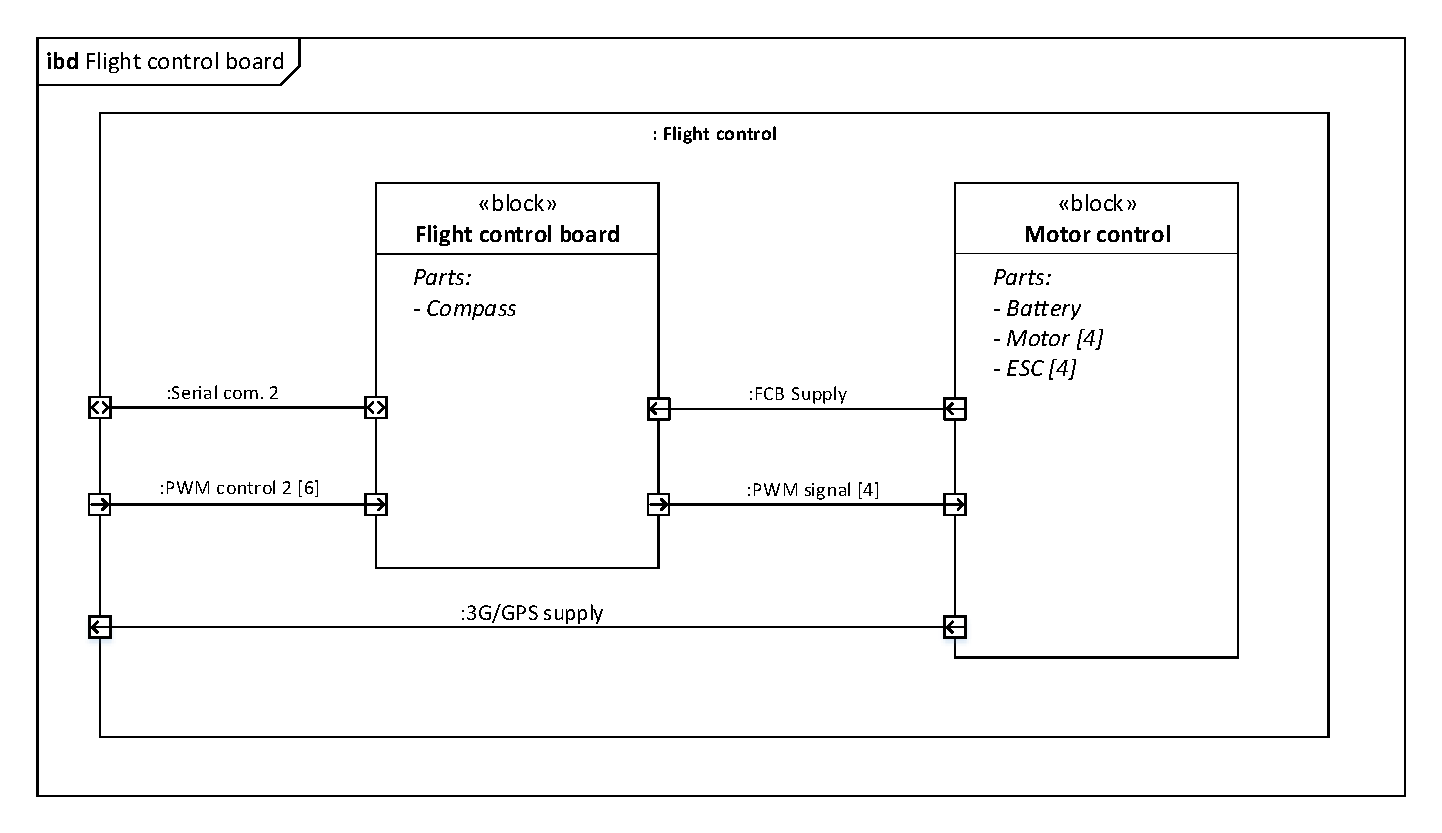
\includegraphics[width=1\textwidth]{Billeder/IBD/ibd5_flightcontrolboard.pdf}
\caption{ibd - flight control board}
\label{fig:ibd_flightcontrolboard}
\end{figure}

\begin{table}[H]
	\centering
		\begin{tabular}{|p{2.5 cm}|p{5.5 cm}|p{2.5 cm}|p{2.5 cm}|} 
		\hline
			\textbf{Signal navn} 	& \textbf{Signal beskrivelse}		& \textbf{Out} 				& \textbf{In}     \\ \hline
			User input 			& Via \textit{webapplication} opsætter bruger ny flyvning eller undersøger tidligere & Bruger 		& Webapplication.			    \\ \hline
			User interface 		& 03-09-14	& KG,RL,AO				& .				\\ \hline
			Flight setup		& 09-09-14	& KG,RL					& .	\\ \hline
			Flight feedback		& 25-08-14	& KG,RL,AO				& .			    \\ \hline
			GPS signal 1		& 03-09-14	& KG,RL,AO				& .				\\ \hline
			GPS signal 2		& 09-09-14	& KG,RL					& .	\\ \hline  
		\end{tabular}
	\caption{Forbindelser IDB 1}
	\label{tab:IDB1}
\end{table}



